% Chapter 12
\section{Introduction to Recurrent Neural Networks}\label{chap:rnn}
\graphicspath{{assets/lec7/}{assets/lec9/}{assets/lec14/}}

\Cref{chap:cnn} showed how architectural bias (convolution/pooling) improves sample efficiency while preserving the same optimization loop. This chapter keeps that loop but changes the axis from space to time: sequence models need memory so present predictions can depend on prior tokens. \Cref{fig:roadmap} flags this as the sequential branch of the neural strand.

\begin{tcolorbox}[summarybox, title={Learning Outcomes}]
\begin{itemize}
    \item Explain why recurrent structures are needed for sequence modeling and contrast them with feedforward nets.
    \item Derive the forward dynamics and backpropagation-through-time (BPTT) updates for vanilla RNN cells.
    \item Recognize practical stabilization techniques (gradient clipping, gating, normalization) that motivate later LSTM/Transformer chapters.
\end{itemize}
\end{tcolorbox}

\begin{tcolorbox}[summarybox, title={Design motif}]
Add recurrence, then train it by unrolling time and reusing the backprop machinery from \Cref{chap:backprop}.
\end{tcolorbox}

The statistical learning chapters (\Crefrange{chap:supervised}{chap:logistic}) established the basic training loop: choose a model class, define a loss, optimize it, and then audit generalization and calibration. The feedforward neural chapters then expanded the model class from linear predictors to multilayer networks (MLPs, RBF networks, and CNNs).

Those architectures are effective for classification, regression, and feature extraction, but they share a structural limitation: information flows strictly from input to output, without an internal state that can store context over time.

\subsection{Motivation for Recurrent Neural Networks}
\label{sec:rnn_motivation_for_recurrent_neural_networks}

Before delving into the architecture and mathematics of RNNs, it is important to understand why feedforward networks are insufficient for certain applications. Consider the following scenario:

\begin{quote}
\textit{You want to predict an output at time $t$ based not only on the input at time $t$, but also on inputs from previous time steps $t-1, t-2, \ldots, t-k$.}
\end{quote}

This is a common situation in many real-world problems, such as:

\begin{itemize}
    \item Time series forecasting (e.g., stock prices, weather data)
    \item Natural language processing (e.g., predicting the next word in a sentence)
    \item Speech recognition and synthesis
    \item Control systems with memory of past states
\end{itemize}

\paragraph{Chapter flow.}
We proceed in one pass: motivate temporal memory, formalize state updates and parameter sharing, derive unrolling/BPTT, then cover stabilization (clipping and gating) before closing with attention as the transition beyond recurrent bottlenecks. Optional reminders are kept near the chapter close so they do not interrupt the derivation arc.

Order carries meaning even in simple settings: if it is Saturday, the next day is Sunday. In language, ``out of the blue'' means something sudden, whereas ``the ball was blue'' refers to color; the sequence makes the difference. In predictive text, ``I want to buy...'' favors a different continuation than ``Write a book about Teddy...'' These examples also highlight variable-length inputs: a review can be three words or three hundred. You can always build a fixed window of past inputs and feed it to a standard MLP, but that approach scales poorly as the history grows and does not share parameters across time.

Feedforward networks treat each input independently and do not have an inherent mechanism to remember or utilize past inputs. To incorporate past information, one might consider explicitly including previous inputs as part of the current input vector, but this approach quickly becomes impractical as the history length grows.

\subsection{Key Idea: State and Memory in RNNs}
\label{sec:rnn_key_idea_state_and_memory_in_rnns}

Recurrent neural networks address this limitation by introducing a \emph{state vector} $\mathbf{h}_t$ that summarizes information from all previous inputs up to time $t$. The state is updated recursively as new inputs arrive, allowing the network to maintain a form of memory.

Formally, at each time step $t$, the RNN receives an input vector $\mathbf{x}_t$ and updates its hidden state $\mathbf{h}_t$ according to a function $f$ parameterized by weights $\theta$:

\begin{align}
    \mathbf{h}_t = f(\mathbf{h}_{t-1}, \mathbf{x}_t; \theta)
    \label{eq:rnn_state_update}
\end{align}

The output $\mathbf{y}_t$ at time $t$ is then computed as a function of the current state:

\begin{align}
    \mathbf{y}_t = g(\mathbf{h}_t; \theta')
    \label{eq:rnn_output}
\end{align}

Here, $f$ and $g$ are typically nonlinear functions implemented by neural network layers, and $\theta, \theta'$ are learned parameters.

\paragraph{Interpretation:} The hidden state $\mathbf{h}_t$ acts as a \emph{summary} or \emph{encoding} of the entire input history $\{\mathbf{x}_1, \mathbf{x}_2, \ldots, \mathbf{x}_t\}$. This allows the network to make predictions that depend on the temporal context, not just the current input.

\paragraph{Parameter sharing across time.} The same weights are reused at each time step. In the simplest formulation there are three learned matrices: \(W_{xh}\) (input to state), \(W_{hh}\) (state to state), and \(W_{hy}\) (state to output). When you unroll the recurrence, these matrices appear at every step, so the model learns a single transition rule rather than a separate set of parameters for each position in the sequence.

Unrolling makes the training graph \(T\) steps deep. Gradients from each time step accumulate onto the shared weights, and the repeated Jacobian products are precisely why long sequences revive the vanishing/exploding gradient issues from deep feedforward networks.
Training this unrolled graph with standard backpropagation is known as \emph{backpropagation through time} (BPTT).

Recurrent neural networks (RNNs) were among the first practical sequence models \citep{Elman1990,Bengio1994}. CNNs from \Cref{chap:cnn} trade recurrence for parallel, spatially shared filters. \Cref{chap:nlp} then supplies the token representations and evaluation lens commonly paired with RNNs, and \Cref{chap:transformers} revisits sequence modeling without recurrence.

\subsection{Comparison with Feedforward Networks}
\label{sec:rnn_comparison_with_feedforward_networks}

To contrast, a feedforward network computes the output at time $t$ as:

\begin{align}
    \mathbf{y}_t = \psi(\mathbf{x}_t; \theta)
    \label{eq:ffn_output}
\end{align}

where $\psi$ is a nonlinear function without any dependence on past inputs. This limits the ability of feedforward networks to model temporal dependencies unless the input vector $\mathbf{x}_t$ explicitly contains past information.

\paragraph{Summary:} RNNs extend feedforward networks by incorporating a recurrent connection that allows information to persist across time steps, enabling modeling of sequences and temporal dynamics.

\begin{tcolorbox}[summarybox, title={Shape reminder}]
We keep the row-major (deep-learning) convention: \(\mathbf{x}_t \in \mathbb{R}^{d_x}\), \(\mathbf{h}_t \in \mathbb{R}^{d_h}\), pre-activation \(\mathbf{a}_t = \mathbf{x}_t W_{xh} + \mathbf{h}_{t-1} W_{hh} + \mathbf{b}_h\), output \(\mathbf{y}_t = \mathbf{h}_t W_{hy} + \mathbf{b}_y\). Column-vector formulations simply transpose the order of factors; all stability conclusions (spectral norms of Jacobian factors) carry over.
\end{tcolorbox}

\paragraph{Roadmap.}\label{sec:rnn_outline_of_this_chapter}
The sequence is: architecture and state updates, unrolling/BPTT, instability sources, stabilization strategies, gated variants, and attention-era transition.

\subsection{Recap: Feedforward Building Blocks}
\label{sec:rnn_recap_feedforward_building_blocks}

\paragraph{Simple RNN at a glance.}
\begin{itemize}
    \item \textbf{Objective:} Minimize cross\hyp{}entropy (or another sequence loss) between targets and \(p_\theta(y_t\mid \mathbf{h}_t)\), with \(\mathbf{h}_t = f(\mathbf{x}_t W_{xh} + \mathbf{h}_{t-1} W_{hh} + b_h)\).
    \item \textbf{Key hyperparameters:} hidden state size, BPTT truncation window, optimizer/learning rate, regularization (dropout, weight decay), and clipping threshold.
    \item \textbf{Defaults:} \(\tanh\) or ReLU activations, hidden size 128--512, Adam or SGD+momentum with clipping, and layer norm or gating (LSTM/GRU) for long sequences.
    \item \textbf{Common pitfalls:} vanishing/exploding gradients on long sequences, too-small hidden states, and train/test mismatch when teacher forcing is not reflected at inference.
\end{itemize}

RNNs reuse the same ingredients as multilayer perceptrons (activations, nonlinear decision boundaries, loss functions, and training heuristics) but wrap them around a temporal axis. \Cref{fig:backprop-computational-graph} from \Cref{chap:backprop} highlights the canonical MLP dataflow along with common activation choices and derivatives that govern gradient flow.

Two-dimensional toy datasets remain useful for reasoning about inductive biases. \Cref{fig:lec7-boundaries} contrasts logistic regression and a shallow MLP on the moons dataset, illustrating how additional hidden units carve nonlinear boundaries that RNN readouts later rely on when decoding the final state.

\begin{figure}[t]
    \centering
    \begin{tikzpicture}
        \begin{groupplot}[
            group style={group size=2 by 1, horizontal sep=1cm},
            width=0.43\linewidth,
            height=0.38\linewidth,
            xmin=-1.2, xmax=1.6,
            ymin=-0.8, ymax=1.4,
            xlabel={$x_1$},
            ylabel={$x_2$},
            axis equal,
            legend style={at={(0.03,0.03)}, anchor=south west, legend columns=2, fill=white, draw=none}
        ]
            \nextgroupplot[title={Logistic regression}]
                \addplot+[only marks, mark=*, color=cbBlue, mark size=1.6pt] coordinates {
                    (0.1,0.4) (0.3,0.8) (-0.1,0.9) (-0.4,0.6) (-0.6,0.2)
                    (-0.3,0.1) (-0.7,0.55) (-0.2,0.35) (0.2,1.0) (0.5,0.6)
                };
                \addlegendentry{Class 1}
                \addplot+[only marks, mark=square*, color=cbOrange, mark size=1.6pt] coordinates {
                    (0.4,-0.2) (0.8,-0.3) (1.0,0.1) (0.6,-0.5) (0.2,-0.4)
                    (-0.2,-0.3) (-0.5,-0.4) (0.9,0.35) (1.2,0.2) (0.6,0.2)
                };
                \addlegendentry{Class 2}
                \addplot[thick, color=black] coordinates {(-1.2,-0.2) (1.6,0.6)};
                \node[anchor=west, font=\scriptsize] at (axis cs:0.9,0.65){$w^\top x + b = 0$};
            \nextgroupplot[title={Shallow MLP}]
                \addplot+[only marks, mark=*, color=cbBlue, mark size=1.6pt] coordinates {
                    (0.1,0.4) (0.3,0.8) (-0.1,0.9) (-0.4,0.6) (-0.6,0.2)
                    (-0.3,0.1) (-0.7,0.55) (-0.2,0.35) (0.2,1.0) (0.5,0.6)
                };
                \addplot+[only marks, mark=square*, color=cbOrange, mark size=1.6pt] coordinates {
                    (0.4,-0.2) (0.8,-0.3) (1.0,0.1) (0.6,-0.5) (0.2,-0.4)
                    (-0.2,-0.3) (-0.5,-0.4) (0.9,0.35) (1.2,0.2) (0.6,0.2)
                };
                \addplot[cbGreen, thick, domain=-1.2:1.4, samples=200]
                    {0.35 + 0.55*sin(deg(2.1*x)) - 0.1*x};
                \node[anchor=west, font=\scriptsize, cbGreen] at (axis cs:0.9,0.95){Nonlinear separator};
        \end{groupplot}
    \end{tikzpicture}
    \caption{Decision boundaries for logistic regression (left) versus a shallow MLP (right). Linear models carve a single hyperplane, whereas hidden units can warp the boundary to follow non-convex manifolds such as the moons dataset. Use it when diagnosing whether representation capacity (not optimization) limits a classifier.}
    \label{fig:lec7-boundaries}
\end{figure}


\Cref{fig:lec7-rnn-unrolled} is the canonical unrolling view used to interpret shared-parameter BPTT updates.

Finally, \Cref{fig:lec7-loss-hyperparams} summarizes two diagnostics: BCE geometry and the effect of learning\hyp{}rate schedules/early stopping.
Here BCE (binary cross\hyp{}entropy) for a binary target $y\in\{0,1\}$ and logit $z$ is $\mathcal{L}(z, y)=\log(1+e^{-z})$ for $y{=}1$ and $\log(1+e^{z})$ for $y{=}0$; the \emph{logit} $z$ is the pre\hyp{}sigmoid score so that $\sigma(z)$ yields the predicted probability. The middle panel contrasts a conservative schedule (smooth decay) with a more aggressive one (faster initial drop but risk of oscillation), and the right panel shows early stopping triggered when validation loss ceases to improve while training loss continues decreasing.
We will reuse these when tuning sequence models, where overfitting appears as a divergence between per\hyp{}token training and validation likelihood.

\begin{tcolorbox}[summarybox, title={Author's note: treat early stopping as the default brake}]
Unless there is a compelling reason to run to numerical convergence, stop as soon as the validation curve flattens while the training curve keeps dropping. Checkpoint the best weights and resume only if new data or regularization changes warrant it. That simple rule prevents most runaway experiments without elaborate hyperparameter sweeps.
\end{tcolorbox}

\begin{figure}[t]
    \centering
    \begin{tikzpicture}
        \begin{groupplot}[
            group style={group size=3 by 1, horizontal sep=1.2cm},
            width=0.32\linewidth, height=0.36\linewidth
        ]
        % BCE vs logit
        \nextgroupplot[
            title={BCE vs logit $z$},
            xlabel={$z$},
            ylabel={$\mathcal{L}$},
            xmin=-6, xmax=6,
            ymin=0, ymax=6,
            legend style={at={(0.97,0.97)}, anchor=north east, fill=white, draw=none}
        ]
            \addplot[cbBlue, thick, samples=200, domain=-6:6] {ln(1+exp(-x))}; \addlegendentry{$y{=}1$}
            \addplot[cbOrange, dashed, thick, samples=200, domain=-6:6] {ln(1+exp(x))}; \addlegendentry{$y{=}0$}
        % Learning-rate effect (schematic loss curves)
        \nextgroupplot[
            title={Learning rate effect},
            xlabel={epoch},
            ylabel={loss},
            xmin=0, xmax=50,
            ymin=0, ymax=1.2,
            legend style={at={(0.97,0.97)}, anchor=north east, fill=white, draw=none}
        ]
            \addplot[cbBlue, thick, samples=100, domain=0:50] {0.2 + 0.9*exp(-x/12)}; \addlegendentry{conservative}
            \addplot[cbPink, dashed, thick, samples=100, domain=0:50] {0.15 + 1.0*exp(-x/6) + 0.05*sin(0.6*x)}; \addlegendentry{aggressive}
        % Early stopping (train vs val)
        \nextgroupplot[
            title={Early stopping},
            xlabel={epoch},
            ylabel={loss},
            xmin=0, xmax=50,
            ymin=0, ymax=1.2,
            legend style={at={(0.97,0.97)}, anchor=north east, fill=white, draw=none}
        ]
            \addplot[cbGreen, thick, samples=100, domain=0:50] {0.1 + 0.9*exp(-x/10)}; \addlegendentry{train}
            % U-shaped validation curve: improves early, then degrades (overfitting).
            \addplot[cbOrange, dashed, thick, samples=200, domain=0:50] {0.25 + 0.7*exp(-x/12) + 0.0004*(x-20)^2}; \addlegendentry{val}
            \addplot[gray!70, dashed] coordinates {(20,0) (20,1.2)};
            \node[font=\scriptsize, anchor=south west, gray!70] at (axis cs:20,0.08) {stop};
        \end{groupplot}
    \end{tikzpicture}
    \ifdefined\HCode
        \caption{Binary cross-entropy geometry (left), effect of learning-rate schedules on loss (middle), and the typical training/validation divergence that motivates early stopping (right). Use it when choosing a learning-rate schedule and interpreting early-stopping signals.}
    \else
        % Avoid inline math in captions; it wraps poorly in some EPUB renderers.
        \caption{Binary cross-entropy geometry (left), effect of learning-rate schedules on loss (middle), and the typical training/validation divergence that motivates early stopping (right). Use it when choosing a learning-rate schedule and interpreting early-stopping signals.}
    \fi
    \label{fig:lec7-loss-hyperparams}
\end{figure}


\begin{tcolorbox}[summarybox, title={LayerNorm and residual RNN tips}]
Layer Normalization~\citep{Ba2016} stabilizes recurrent dynamics by normalizing each hidden vector \(\mathbf{h}_t\) across features before applying the nonlinearity; unlike BatchNorm it works with batch size 1 and handles variable-length sequences gracefully. Residual RNN stacks (adding the input of a layer back to its output) keep gradients flowing even when depth increases, mirroring the skip-connections that make deep CNNs trainable. Together, LayerNorm + residual links curb exploding/vanishing gradients and are the default when building multi-layer RNN/LSTM stacks.
\end{tcolorbox}

\paragraph{Historical Note: Hopfield Networks}

An early influential recurrent network is the Hopfield network \citep{Hopfield1982}, which is a form of associative memory. Unlike modern RNNs, Hopfield networks have symmetric weights and are designed to converge to stable states representing stored patterns. While Hopfield networks are not directly used for sequence modeling, they helped establish the energy-based viewpoint that reappears in later recurrent and attention-based models.

Bidirectional extensions run two RNNs in opposite directions and concatenate their states; they are widely used in encoders for labeling tasks when the full context is available.

\subsection{Input--output configurations and mathematical formulation}
\label{sec:rnn_input_output_configurations_and_mathematical_formulation}

RNNs can map sequences to sequences in several ways:
\begin{itemize}
    \item Many-to-one (e.g., sentiment classification): consume \(\mathbf{x}_{1: T}\), emit one label after the final state.
    \item One-to-many (e.g., conditional generation): condition on a context vector, then autoregressively emit a sequence.
    \item Many-to-many (e.g., tagging, ASR): emit \(\mathbf{y}_t\) at every step; encoder--decoder variants compress \(\mathbf{x}_{1: T}\) then decode.
    \item Bidirectional encoders: run a forward and backward RNN and concatenate the states for sequence labeling or as encoder context.
    \end{itemize}

Consider an input sequence \(\{\mathbf{x}_1, \mathbf{x}_2, \ldots, \mathbf{x}_T\}\), where each \(\mathbf{x}_t \in \mathbb{R}^d\). The RNN computes hidden states \(\{\mathbf{h}_1, \mathbf{h}_2, \ldots, \mathbf{h}_T\}\) and outputs \(\{\mathbf{y}_1, \mathbf{y}_2, \ldots, \mathbf{y}_T\}\) as follows:
\begin{align}
\mathbf{h}_0 &= \mathbf{0} \quad \text{(initial hidden state)} \\
\mathbf{h}_t &= f(\mathbf{x}_t W_{xh} + \mathbf{h}_{t-1} W_{hh} + b_h), \quad t=1,\ldots, T \label{eq:rnn_hidden_state}\\
\mathbf{y}_t &= g(\mathbf{h}_t W_{hy} + b_y), \quad t=1,\ldots, T \label{eq:rnn_output_state}
\end{align}

\begin{tcolorbox}[summarybox, title={Shapes and masks (batch $B$, time $T$)}]
Inputs \(X \in \mathbb{R}^{B\times T \times d_x}\); hidden states \(H \in \mathbb{R}^{B\times T \times d_h}\); logits \(Y \in \mathbb{R}^{B\times T \times d_o}\). Parameters (row-major): \(W_{xh}\in\mathbb{R}^{d_x\times d_h}\), \(W_{hh}\in\mathbb{R}^{d_h\times d_h}\), \(W_{hy}\in\mathbb{R}^{d_h\times d_o}\), biases \(b_h\in\mathbb{R}^{d_h}\), \(b_y\in\mathbb{R}^{d_o}\).\\
Padding mask \(M\in\{0,1\}^{B\times T}\): loss \(L=\sum_{b, t} M_{b, t}\,\text{CE}(\hat y_{b, t}, y_{b, t})/\sum_{b, t} M_{b, t}\). Masks preview the padding/causal masks detailed in \Cref{chap:transformers}.
\end{tcolorbox}
\paragraph{Unrolling and shared weights.}
The cleanest way to understand recurrence is to \emph{unroll time}: the same cell is applied repeatedly, reusing the same parameters at each step. Training then becomes ordinary backpropagation on the unrolled computation graph, with gradients accumulated across every copy of the shared weights (backpropagation through time, BPTT).

\subsection{Mathematical Formulation of a Simple RNN Cell}
\label{sec:rnn_mathematical_formulation_of_a_simple_rnn_cell}

Consider a simple RNN cell with the following update equations:
\begin{align}
    \mathbf{h}_t &= \sigma_h \left( \mathbf{x}_t \mathbf{W}_{xh} + \mathbf{h}_{t-1} \mathbf{W}_{hh} + \mathbf{b}_h \right), \label{eq:simple_rnn_hidden} \\
    \mathbf{y}_t &= \sigma_y \left( \mathbf{h}_t \mathbf{W}_{hy} + \mathbf{b}_y \right). \label{eq:simple_rnn_output}
\end{align}
\begin{figure}[t]
    \centering
    \begin{tikzpicture}[
        font=\small\sffamily,
        >=Latex,
        node distance=2.4cm,
        box/.style={draw, rounded corners, minimum width=1.8cm, minimum height=0.9cm},
        arrow/.style={->, thick}
    ]
        % Nodes
        \node[box] (h1) at (0,0) {$h_{t-1}$};
        \node[box, right=of h1] (h2) {$h_{t}$};
        \node[box, right=of h2] (h3) {$h_{t+1}$};
        \node (x1) at (0,-1.2) {$x_{t-1}$};
        \node (x2) at (h2|-x1) {$x_{t}$};
        \node (x3) at (h3|-x1) {$x_{t+1}$};
        \node (y1) at (0,1.2) {$y_{t-1}$};
        \node (y2) at (h2|-y1) {$y_{t}$};
        \node (y3) at (h3|-y1) {$y_{t+1}$};
        % Arrows
        \draw[arrow] (h1) -- node[above, font=\scriptsize] {$\mathbf{W}_{hh}$} (h2);
        \draw[arrow] (h2) -- (h3);
        \draw[arrow] (x1) -- node[midway, right, font=\scriptsize, xshift=1mm] {$\mathbf{W}_{xh}$} (h1);
        \draw[arrow] (x2) -- node[midway, right, font=\scriptsize, xshift=1mm] {$\mathbf{W}_{xh}$} (h2);
        \draw[arrow] (x3) -- node[midway, right, font=\scriptsize, xshift=1mm] {$\mathbf{W}_{xh}$} (h3);
        \draw[arrow] (h1) -- node[midway, right, font=\scriptsize, xshift=1mm] {$\mathbf{W}_{hy}$} (y1);
        \draw[arrow] (h2) -- node[midway, right, font=\scriptsize, xshift=1mm] {$\mathbf{W}_{hy}$} (y2);
        \draw[arrow] (h3) -- node[midway, right, font=\scriptsize, xshift=1mm] {$\mathbf{W}_{hy}$} (y3);

        % Shared-parameter annotation: brace anchored to the left/right cells so it
        % stays aligned if the figure spacing changes.
        \coordinate (braceL) at ($(h1.south west)+(0,-12mm)$);
        \coordinate (braceR) at ($(h3.south east)+(0,-12mm)$);
        \draw[decorate, decoration={brace, amplitude=5pt}] (braceL) -- node[midway, below=10pt]{\scriptsize shared parameters across the unrolled sequence} (braceR);
    \end{tikzpicture}
    \caption{Unrolling an RNN reveals repeated application of the same parameters across time steps. This view motivates backpropagation through time (BPTT), which accumulates gradients through every copy before updating the shared weights. Use it when translating a recurrent cell into an explicit computation graph for training.}
    \label{fig:lec7-rnn-unrolled}
\end{figure}

\subsection{Recurrent Neural Network (RNN) Architectures and Loss Computation}
\label{sec:rnn_recurrent_neural_network_rnn_architectures_and_loss_computation}

Recall from previous discussions that the loss function for classification tasks often involves cross\hyp{}entropy terms of the form:
\begin{equation}
\mathcal{L} = - \sum_{i} y_i \log \hat{y}_i,
\label{eq:auto_rnn_5a12cb8d8f}
\end{equation}
where \( y_i \) is the true label (often one-hot encoded) and \( \hat{y}_i \) is the predicted probability for class \( i \). When \( \hat{y} = y \), the loss is zero, indicating perfect prediction.

In the context of RNNs, the total loss over a sequence is typically the sum of losses at each time step:
\begin{equation}
\mathcal{L}_{\text{total}} = \sum_{t=1}^T \mathcal{L}_t,
\label{eq:auto_rnn_04c572b36d}
\end{equation}
where \( T \) is the sequence length.

\paragraph{Forward and Backward Passes in RNNs}

The forward pass involves propagating inputs through the network over time steps \( t = 1, \ldots, T \), producing outputs \( \hat{y}_t \) at each step. After computing the loss, the backward pass computes gradients with respect to parameters by backpropagating errors through time, a process known as \emph{Backpropagation Through Time} (BPTT).

BPTT unfolds the RNN across time steps and applies standard backpropagation through this unrolled network. The key insight is that parameters are shared across time steps, so gradients accumulate contributions from all time steps; \Cref{fig:lec7-bptt} highlights the simultaneous forward flow (black) and backward gradients (pink) that piggyback across every copy.

\begin{tcolorbox}[summarybox, title={Truncated BPTT in practice}]
Unroll \(K\) steps, accumulate loss, backprop through those \(K\) steps, then detach the hidden state to stop graph growth:
\begin{verbatim}
h = h0
for t in range(T):
    h, yhat = rnn(x[t], h)
    loss += mask[t] * CE(yhat, y[t])
    if (t+1) % K == 0:
        loss.backward()
        clip_grad_norm_(model.parameters(), tau)
        opt.step(); opt.zero_grad()
        h = h.detach()  # carry state, drop graph
\end{verbatim}
Choose \(K\) to balance memory and credit assignment (common range: 20--100 steps).
\end{tcolorbox}

\begin{tcolorbox}[summarybox, title={Vanilla RNN cell (forward + BPTT)}]
\begin{verbatim}
# Forward for a sequence {x_t, y_t}
h_0 = 0
for t = 1..T:
    pre_h = h_{t-1} W_hh + x_t W_xh + b_h
    h_t  = tanh(pre_h)
    yhat_t = h_t W_hy + b_y

# Backward (BPTT with optional truncation K)
delta_pre_next = 0
for t = T..1:
    delta_y = grad_loss(yhat_t, y_t)
    grad_W_hy += h_t^T delta_y
    grad_b_y += delta_y
    delta_h = delta_y W_hy^T + delta_pre_next W_hh^T
    delta_pre = delta_h .* (1 - h_t^2)
    grad_W_hh += h_{t-1}^T delta_pre
    grad_W_xh += x_t^T delta_pre
    grad_b_h += delta_pre
    delta_pre_next = delta_pre
    if t < T-K: break  # truncated BPTT
\end{verbatim}
Use gradient clipping (e.g., clip the global norm of parameter gradients) and layer/batch normalization when sequences are long to avoid exploding/vanishing gradients.
\end{tcolorbox}

The element-wise product in the backward step corresponds to the Hadamard factors described in the derivation in \Cref{chap:mlp}; we write it as \texttt{.*} to align with NumPy/Matlab notation.
\paragraph{Code--math dictionary.}
In code blocks we use ASCII identifiers such as \texttt{h\_t}, \texttt{W\_hh}, and \texttt{b\_h}; in equations the same objects appear as \(\mathbf{h}_t\), \(\mathbf{W}_{hh}\), and \(\mathbf{b}_h\) (boldface for vectors/matrices, subscripts for time and role). Detailed algebraic derivations (forward/backward passes and gradient expressions) appear in \Crefrange{eq:simple_rnn_hidden}{eq:simple_rnn_output}.

\begin{figure}[t]
    \centering
    \begin{tikzpicture}[
        font=\small\sffamily,
        >=Latex,
        arrow/.style={->, thick}
    ]
        % forward chain
        \foreach \i in {0,...,4} {
            \node[draw, rounded corners, minimum width=1.2cm, minimum height=0.7cm] (h\i) at (2*\i,0) {$h_{t+\i}$};
            \node (x\i) at (2*\i,-1.0) {$x_{t+\i}$};
            \draw[arrow] (x\i) -- (h\i);
        }
        \foreach \i/\j in {0/1,1/2,2/3,3/4} {\draw[arrow] (h\i) -- (h\j);}
        % backward (gradient) arrows
        \foreach \i/\k in {1/0,2/1,3/2,4/3} {
            \draw[cbPink, <-, thick] (h\i.north).. controls +(0,1.0) and +(0,1.0).. node[above, pos=0.5]{\scriptsize $\partial\mathcal{L}/\partial h_{t+\i}$} (h\k.north);
        }
        % shared parameters note
        \node at (4,-2.0) {\scriptsize shared $(\mathbf{W}_{hh}, \mathbf{W}_{xh}, \mathbf{W}_{hy})$ across time};
    \end{tikzpicture}
    \caption{Backpropagation through time (BPTT): unrolled forward pass (black) and backward gradients (pink) through time. Use it when reasoning about truncation windows and why long histories strain gradient flow.}
    \label{fig:lec7-bptt}
\end{figure}


\paragraph{Vanishing and Exploding Gradients}

Because each gradient term contains products of Jacobians such as
\[
\frac{\partial \mathbf{h}_t}{\partial \mathbf{h}_{t-1}} = \mathrm{diag}\!\big( f'(\mathbf{a}_t) \big)\,\mathbf{W}_{hh}^{\top},
\]
with pre\hyp{}activation \(\mathbf{a}_t=\mathbf{x}_t\mathbf{W}_{xh}+\mathbf{h}_{t-1}\mathbf{W}_{hh}+\mathbf{b}_h\) and elementwise nonlinearity \(f\), long sequences multiply many such factors. Here \(\mathbf{W}_{hh}\in\mathbb{R}^{d_h\times d_h}\) and \(\mathrm{diag}\big(f'(\mathbf{a}_t)\big)\in\mathbb{R}^{d_h\times d_h}\), so the Jacobian \(\partial \mathbf{h}_t/\partial \mathbf{h}_{t-1}\) is a \(d_h\times d_h\) matrix. If the spectral norm of each factor is below one the product decays exponentially (vanishing); norms above one cause growth (exploding). \Cref{fig:lec7-vanishing} illustrates both behaviors across time. Practical remedies include gradient clipping, orthogonal or unitary recurrent matrices, layer normalization, and gated architectures (LSTM/GRU) that introduce additive memory paths.
Empirically, vanilla RNNs often fail to preserve dependencies beyond roughly 5--10 steps in language tasks, which is why gated cells became the default for longer sequences.
\begin{figure}[t]
    \centering
    \includegraphics[width=0.72\linewidth]{lec7_vanish_explode}
    \caption{Vanishing (blue) versus exploding (orange) gradients on a log scale. The gray strip highlights the stability band; the inset reminds readers that repeated Jacobian products either shrink gradients (thin blue arrows) or amplify them (thick orange arrows). Use it when diagnosing why long-range dependencies fail to train.}
    \label{fig:lec7-vanishing}
\end{figure}


\paragraph{Parameter Updates}

At each time step, the gradient of the loss with respect to parameters (e.g., weights \( W \)) depends on the chain of partial derivatives through the network states:
\begin{equation}
\frac{\partial \mathcal{L}}{\partial W} = \sum_{t=1}^T \frac{\partial \mathcal{L}_t}{\partial W}.
\label{eq:auto_rnn_228bc3ab0f}
\end{equation}
Because of parameter sharing, the same \( W \) influences multiple time steps, and the total gradient is the sum over these contributions.

\subsection{Stabilizing Recurrent Training}
\label{sec:rnn_stabilizing_recurrent_training}

\paragraph{Gradient clipping.} A practical safeguard is to clip the global norm of the gradient when it exceeds a threshold. \Cref{fig:lec7-clipping} shows how clipping prevents the exploding case from destabilizing optimization while leaving the vanishing regime untouched. Orthogonal or unitary initializations for the recurrent weight matrix \(W_{hh}\) are another common trick: because orthogonal matrices preserve Euclidean norms, gradients neither explode nor vanish in the very early stages of training (before nonlinearities and data\hyp{}dependent effects accumulate).

\begin{tcolorbox}[summarybox, title={Stability defaults in practice}]
Spectral norm \(\|\mathbf{W}_{hh}\|_2 \approx 1\) keeps gradients roughly stable over tens of steps; clipping thresholds \(\tau \in [0.5, 5]\) are sensible defaults when sequences are long. BatchNorm inside the recurrent loop is rarely helpful; prefer LayerNorm or gating to stabilize dynamics.
\par\smallskip
\textbf{Author's note: do not fight vanilla RNNs.} If your task needs dependencies longer than a handful of steps, do not over-tune a plain RNN. Start with clipping and a sensible truncation window, but move to GRU/LSTM once long-range information vanishes.
\end{tcolorbox}

\paragraph{Dropout in RNNs.} Variational/recurrent dropout applies the same dropout mask at every time step to avoid injecting temporal noise \citep{Gal2016,Semeniuta2016}; zoneout preserves hidden units stochastically instead of zeroing them \citep{Krueger2016}. Standard per-time-step dropout often harms sequence retention.

\begin{figure}[t]
    \centering
    \begin{tikzpicture}
        \begin{groupplot}[
            group style={group size=2 by 1, horizontal sep=1.6cm},
            width=0.44\linewidth,
            height=0.35\linewidth,
            xmin=0, xmax=80,
            xlabel={Iteration},
            grid=both,
            minor tick num=1,
            xlabel style={yshift=4pt}
        ]
            \nextgroupplot[
                ylabel={$\|\mathbf{g}\|$},
                ymin=0, ymax=20,
                legend style={at={(0.02,0.95)}, anchor=north west},
                ytick={0,5,10,15,20}
            ]
                \addplot[cbOrange, thick, smooth] table {
                x y
                0 4
                10 5
                20 7
                30 10
                40 13
                50 16
                60 18
                70 17
                80 19
                };
                    \addlegendentry{Unclipped}
                    \addplot[cbGreen, thick, smooth] table {
                    x y
                    0 4
                    10 4.5
                    20 5
                    30 5.7
                    40 6.5
                    50 6.5
                    60 6.5
                    70 6.5
                    80 6.5
                    };
                    \addlegendentry{Clipped at $\tau$}
                    \draw[gray!40, thick, dashed] (axis cs:0,6.5) -- (axis cs:80,6.5)
                        node[pos=0.98, anchor=south east, font=\scriptsize]{threshold $\tau$};
            \nextgroupplot[
                ylabel={Training loss},
                ymin=0.2, ymax=1.2,
                ytick={0.2,0.4,0.6,0.8,1.0,1.2}
            ]
                \addplot[cbOrange, thick, smooth] table {
                x y
                0 1.05
                10 0.9
                20 0.85
                30 0.92
                40 0.95
                50 1.0
                60 1.05
                70 1.1
                80 1.12
                };
                \addplot[cbGreen, thick, smooth] table {
                x y
                0 1.05
                10 0.92
                20 0.8
                30 0.68
                40 0.6
                50 0.55
                60 0.5
                70 0.48
                80 0.46
                };
        \end{groupplot}
    \end{tikzpicture}
    % Avoid inline math in captions; it wraps poorly in some EPUB renderers.
    \caption{Gradient norms (left) explode without clipping (orange) but remain bounded when the global norm is clipped at tau (green). Training loss (right) stabilizes as a result. Use it when setting clipping thresholds to stabilize training without freezing learning.}
    \label{fig:lec7-clipping}
\end{figure}


\paragraph{Teacher forcing and scheduled sampling.} Sequence-to-sequence models frequently feed the ground-truth token back into the decoder during training (teacher forcing) to accelerate convergence. \Cref{fig:lec7-teacher-forcing} contrasts this regime with free-running inference: teacher forcing injects gold tokens at every step, whereas inference conditions the decoder on its own predictions. This mismatch is precisely what scheduled-sampling curricula aim to mitigate \citep{Bengio2015}.

\begin{figure}[t]
\centering
\resizebox{0.92\linewidth}{!}{%
\begin{tikzpicture}[
    x=2.4cm,
    y=1cm,
    font=\small\sffamily,
    >=Latex,
    dec/.style={
        draw, rounded corners=4pt, thick, fill=cbBlue!15,
        minimum width=1.9cm, minimum height=1.0cm,
        align=center
    },
    arrow/.style={->, thick},
    gold/.style={->, thick, cbGreen},
    orange/.style={->, thick, cbOrange}
]

% ==== (a) Teacher forcing ====
\node at (-0.8,2.1) {(a) Teacher forcing};

\node[dec] (d1) at (0,1.2) {$f_\theta$};
\node[dec, right=1 of d1] (d2) {$f_\theta$};
\node[dec, right=1 of d2] (d3) {$f_\theta$};
\node[dec, right=1 of d3, minimum width=1.6cm] (d4) {$f_\theta$};

\node at (-0.8,1.55) {$h_{t-1}$};
\draw[arrow] (-0.55,1.2) -- (d1.west);

\draw[arrow] (d1) -- (d2) node[midway, above=3pt] {\scriptsize distribution};
\draw[arrow] (d2) -- (d3) node[midway, above=3pt] {\scriptsize distribution};
\draw[arrow] (d3) -- (d4);

% gold targets injected upward
\draw[gold] ($(d1.south)+(0,-0.75)$) node[below] {$y_{t-1}$} -- (d1.south);
\draw[gold] ($(d2.south)+(0,-0.75)$) node[below] {$y_t$} -- (d2.south);
\draw[gold] ($(d3.south)+(0,-0.75)$) node[below] {$y_{t+1}$} -- (d3.south);

% ellipsis after fourth block
\node at ($(d4)+(0.6,0)$) {\color{gray}$\cdots$};

% ==== (b) Inference ====
\node at (-0.8,0.1) {(b) Inference};

\node[dec] (s1) at (0,-0.6) {$f_\theta$};
\node[dec, right=1 of s1] (s2) {$f_\theta$};
\node[dec, right=1 of s2] (s3) {$f_\theta$};
\node[dec, right=1 of s3, minimum width=1.6cm] (s4) {$f_\theta$};

\node at (-0.8,-0.25) {$h_{t-1}$};
\draw[arrow] (-0.55,-0.6) -- (s1.west);

\draw[arrow] (s1) -- (s2) node[midway, above=3pt] {\scriptsize sampled token};
\draw[arrow] (s2) -- (s3) node[midway, above=3pt] {\scriptsize sampled token};
\draw[arrow] (s3) -- (s4);

% autoregressive tokens injected upward
\draw[orange] ($(s1.south)+(0,-0.75)$) node[below] {$\langle \text{START}\rangle$} -- (s1.south);
\draw[orange] ($(s2.south)+(0,-0.75)$) node[below] {$\hat y_t$} -- (s2.south);
\draw[orange] ($(s3.south)+(0,-0.75)$) node[below] {$\hat y_{t+1}$} -- (s3.south);

\node at ($(s4)+(0.6,0)$) {\color{gray}$\cdots$};

\end{tikzpicture}
}%

\caption{Teacher forcing vs.\ inference in a sequence-to-sequence decoder. Gold arrows show supervised targets; orange arrows highlight autoregressive feedback that motivates scheduled sampling. Use it when diagnosing train/test mismatch from teacher forcing.}
\label{fig:lec7-teacher-forcing}
\end{figure}


\paragraph{Gated cells.} LSTMs \citep{Hochreiter1997,Gers2000} and GRUs \citep{Cho2014} alleviate vanishing gradients by introducing additive memory paths guarded by gates. \Cref{fig:lec7-lstm,fig:lec7-gru} present the canonical cell diagrams used later in the chapter when deriving the update equations. Intuitively, LSTM forget/input/output gates control retention, writing, and exposure of the memory \(c_t\); GRU update/reset gates interpolate between \(\mathbf{h}_{t-1}\) and a candidate \(\tilde{\mathbf{h}}_t\) and decide how much past context influences the candidate. In an LSTM, the state updates as \(c_t = f_t \odot c_{t-1} + i_t \odot \tilde c_t\) and \(\mathbf{h}_t = o_t \odot \tanh(c_t)\). In a GRU, the hidden state updates as \(\mathbf{h}_t = (1-z_t)\odot \mathbf{h}_{t-1} + z_t \odot \tilde{\mathbf{h}}_t\), with the reset gate \(r_t\) shaping the candidate computation. In both figures, \(\mathbf{x}_t\) denotes the input at time \(t\), and \(\mathbf{h}_{t-1}\) / \(c_{t-1}\) denote the carried state(s).

% LSTM cell: clean routing (no overlaps/crossings; no ambiguous "buses")
% Use an aggressive top-float spec so this can stack with the following GRU cell
% before the summary boxes (avoids the "box jumps ahead, GRU spills to next page" regression).
\begin{figure}[!t]
    \centering
    % Local palette for this diagram (match Figure 52's GRU palette).
    \definecolor{lstmCbBlue}{RGB}{218, 232, 252}
    \definecolor{lstmCbOrange}{RGB}{255, 230, 204}
    \definecolor{lstmCbGray}{RGB}{235, 235, 235}
    \definecolor{lstmArrowGray}{RGB}{100, 100, 100}
    \noindent\resizebox{0.85\textwidth}{!}{%
        \begin{tikzpicture}[
            x=1cm, y=1cm,
            font=\small\sffamily,
            >={Stealth[round, length=2.5mm, width=1.75mm]},
            state/.style={circle, draw, line width=1pt, minimum size=11mm, inner sep=0pt},
            gate/.style={rectangle, rounded corners=3mm, draw, line width=0.8pt,
                fill=lstmCbBlue, minimum width=18mm, minimum height=9mm, align=center},
            cand/.style={rectangle, rounded corners=3mm, draw, line width=0.8pt,
                fill=lstmCbOrange, minimum width=22mm, minimum height=10mm, align=center},
            func/.style={rectangle, rounded corners=2mm, draw, line width=0.8pt,
                fill=lstmCbGray, minimum width=15mm, minimum height=8mm, align=center},
            op/.style={circle, draw, line width=0.8pt, minimum size=7mm, inner sep=0pt, fill=white},
            flow/.style={->, line width=1.2pt, black, rounded corners=5pt, shorten >=1pt},
            lane/.style={->, line width=1.0pt, lstmArrowGray, rounded corners=5pt, shorten >=1pt},
            connect/.style={circle, fill=black, inner sep=0pt, minimum size=4pt}
        ]

            % --- 1. THE HIGHWAY (Top Cell State) ---
            \node[state] (cprev) at (-1.5, 4.0) {$c_{t-1}$};
            \node[op]    (mulF)  at (4.5, 4.0)  {$\odot$};
            \node[op]    (addI)  at (8.0, 4.0)  {$+$};
            \node[state] (ct)    at (13.0, 4.0) {$c_t$};

            % --- 2. INPUTS (Bottom) ---
            \node[state] (hprev) at (-1.5, 0.5) {$h_{t-1}$};
            \node[state] (xt)    at (-1.5,-3.5) {$x_t$};

            % --- 3. GATES STACK (Define positions first) ---
            \node[gate] (ft) at (4.5, 1.5) {$f_t$\\\scriptsize $\sigma$};
            \node[gate] (it) at (4.5, -0.5) {$i_t$\\\scriptsize $\sigma$};
            \node[cand] (ctilde) at (4.5, -2.5) {$\tilde c_t$\\[-2pt]\scriptsize $\tanh$};
            \node[gate] (ot) at (4.5, -4.5) {$o_t$\\\scriptsize $\sigma$};

            % --- 4. AFFINE BLOCK ---
            \node[func, minimum height=7.2cm, minimum width=1.8cm] (affine) at (1.5, -1.5) {\scriptsize Affine};

            % --- 5. LOGIC OPERATORS ---
            \node[op] (mulI) at (8.0, -1.5) {$\odot$};
            \node[cand] (tanhC) at (11.0, 0.5) {$\tanh$};
            \node[op]   (mulO)  at (11.0, -4.5) {$\odot$};
            \node[state] (ht)    at (13.0, -4.5) {$h_t$};
            \node[connect] (cSplit) at (11.0, 4.0) {};

            % ================= CONNECTIONS =================

            % --- INPUTS -> AFFINE ---
            \draw[flow] (hprev) -- (hprev -| affine.west);
            \draw[flow] (xt) -- (xt -| affine.west);

            % --- AFFINE -> GATES ---
            \draw[lane] (affine.east |- ft) -- (ft.west);
            \draw[lane] (affine.east |- it) -- (it.west);
            \draw[lane] (affine.east |- ctilde) -- (ctilde.west);
            \draw[lane] (affine.east |- ot) -- (ot.west);

            % --- GATE LOGIC ---
            \draw[lane] (ft.north) -- (mulF.south);

            \draw[lane] (it.east) -| (mulI.north);
            \draw[flow] (ctilde.east) -| (mulI.south);
            \draw[flow] (mulI.north) -- (addI.south);

            \draw[flow] (cprev) -- (mulF);
            \draw[flow] (mulF) -- (addI);
            \draw[flow, -] (addI) -- (cSplit);
            \draw[flow] (cSplit) -- (ct);

            % --- OUTPUT LOGIC ---
            \draw[flow] (cSplit) -- (tanhC.north);
            \draw[flow] (tanhC.south) -- (mulO.north);
            \draw[lane] (ot.east) -- (mulO.west);
            \draw[flow] (mulO.east) -- (ht.west);

        \end{tikzpicture}%
    }
        \ifdefined\HCode
            \caption{Long Short-Term Memory (LSTM) cell \citep{Hochreiter1997,Gers2000}. Use it when mapping gates and the cell state to the gradient-flow path.}
        \else
            \caption{Long Short-Term Memory (LSTM) cell \citep{Hochreiter1997,Gers2000}. Use it when mapping gates and the cell state to the gradient-flow path.}
        \fi
    \label{fig:lec7-lstm}
\end{figure}


% GRU cell (based on the provided reference TikZ, with explicit (1-z_t) block).
% Matches: h_t = (1-z_t)\odot h_{t-1} + z_t \odot \tilde h_t.
\begin{figure}[!t]
    \centering
    % Local palette for this diagram (avoid clobbering global cbBlue/cbOrange used elsewhere).
    \definecolor{gruCbBlue}{RGB}{218, 232, 252}
    \definecolor{gruCbOrange}{RGB}{255, 230, 204}
    \definecolor{gruCbGray}{RGB}{235, 235, 235}
    \definecolor{gruArrowGray}{RGB}{100, 100, 100}
    \noindent\resizebox{0.85\textwidth}{!}{%
        \begin{tikzpicture}[
            x=1cm, y=1cm,
            font=\small\sffamily,
            >={Stealth[round, length=2.5mm, width=1.75mm]},
            state/.style={circle, draw, line width=1pt, minimum size=11mm, inner sep=0pt},
            gate/.style={rectangle, rounded corners=3mm, draw, line width=0.8pt,
                fill=gruCbBlue, minimum width=18mm, minimum height=9mm, align=center},
            cand/.style={rectangle, rounded corners=3mm, draw, line width=0.8pt,
                fill=gruCbOrange, minimum width=22mm, minimum height=10mm, align=center},
            func/.style={rectangle, rounded corners=2mm, draw, line width=0.8pt,
                fill=gruCbGray, minimum width=15mm, minimum height=8mm, align=center},
            op/.style={circle, draw, line width=0.8pt, minimum size=7mm, inner sep=0pt, fill=white},
            flow/.style={->, line width=1.2pt, black, rounded corners=5pt, shorten >=1pt},
            lane/.style={->, line width=1.0pt, gruArrowGray, rounded corners=5pt, shorten >=1pt},
            connect/.style={circle, fill=black, inner sep=0pt, minimum size=4pt}
        ]

            % --- Nodes ---
            \node[state] (hprev) at (-1.5, 2.0) {$h_{t-1}$};
            \node[state] (x)     at (-1.5,-2.0) {$x_t$};

            \node[func] (affg) at (2.5, 0) {\scriptsize affine};

            \node[gate] (zt) at (5.5, 1.2) {$z_t$\\\scriptsize $\sigma$};
            \node[gate] (rt) at (5.5,-1.2) {$r_t$\\\scriptsize $\sigma$};

            \node[op] (mulr) at (8.0, -1.2) {$\odot$};

            \node[func] (affh)   at (9.8, -1.2) {\scriptsize affine};
            \node[cand] (htilde) at (12.5, -1.2) {$\tilde h_t$\\[-2pt]\scriptsize $\tanh$};

            \node[gate] (oneMinusZ) at (8.0, 3.2) {$1-z_t$};

            \node[op] (mulPrev) at (12.5, 3.2) {$\odot$};
            \node[op] (mulNew)  at (12.5, 0.5) {$\odot$};

            \node[op] (addh)    at (15.0, 0.5) {$+$};

            \node[state] (ht) at (17.0, 0.5) {$h_t$};
            \node[state] (yt) at (17.0,-1.5) {$y_t$};

            % --- SPLIT POINTS ---
            \node[connect] (hSplit) at (0.5, 2.0) {};
            \node[connect] (xSplit) at (0.5, -2.0) {};
            \node[connect] (zSplit) at (7.0, 1.2) {};

            % --- ROUTING ---
            \draw[flow, -] (hprev) -- (hSplit);
            \draw[flow, -] (x) -- (xSplit);

            % Control Lines (Inputs to gates)
            \draw[lane] (hSplit) |- ($(affg.west)+(0,0.15)$);
            \draw[lane] (xSplit) |- ($(affg.west)+(0,-0.15)$);

            \draw[lane] (affg.east) -- ++(0.5,0) |- (zt.west);
            \draw[lane] (affg.east) -- ++(0.5,0) |- (rt.west);

            % Gate Logic Outputs
            \draw[lane, -] (zt) -- (zSplit);
            \draw[lane] (zSplit) -| (oneMinusZ.south);
            \draw[lane] (zSplit) |- (mulNew.west);
            \draw[lane] (rt) -- (mulr);

            % --- MAIN DATA PATHS ---

            % 1. H_prev to Reset Mixer
            % Route: Right to x=4.0 (gap between affine and gates) -> down to y=0 -> right -> down
            \draw[flow] (hSplit) -- (4.0, 2.0) -- (4.0, 0.0) -- (8.0, 0.0) -- (mulr.north);

            % 2. X to Candidate Mixer
            \draw[flow] (xSplit) -| (affh.south);

            % 3. H_prev to Preservation Mixer (High road)
            \draw[flow] (hSplit) -- ++(0, 2.5) -| (mulPrev.north);

            % --- OPERATIONS ---
            \draw[lane] (oneMinusZ.east) -- (mulPrev.west);
            \draw[flow] (mulr) -- (affh);
            \draw[flow] (affh.east) -- (htilde.west);

            \draw[flow] (htilde.north) -- (mulNew.south);

            \draw[flow] (mulPrev.east) -| (addh.north);
            \draw[flow] (mulNew.east) -- (addh.west);

            \draw[flow] (addh) -- (ht);
            \draw[flow] (ht) -- (yt);

        \end{tikzpicture}%
    }
    \ifdefined\HCode
    \caption{Gated Recurrent Unit (GRU) cell \citep{Cho2014}. Use it when comparing gating to vanilla recurrence and to LSTM-style memory.}
    \else
    \caption{Gated Recurrent Unit (GRU) cell \citep{Cho2014}. Use it when comparing gating to vanilla recurrence and to LSTM-style memory.}
    \fi
    \label{fig:lec7-gru}
\end{figure}


        % Keep the cell diagrams together and prevent the following non-float boxes from
        % appearing before a deferred figure.
            \FloatBarrier
            \clearpage

            \begin{tcolorbox}[summarybox, title={Vanilla RNN vs.\ GRU vs.\ LSTM}]
\textbf{Vanilla RNN:} Single hidden state \(\mathbf{h}_t\) updated via \(\mathbf{h}_t=f(\mathbf{x}_tW_{xh}+\mathbf{h}_{t-1}W_{hh}+b_h)\); simplest and parameter\hyp{}efficient but most prone to vanishing/exploding gradients on long sequences.\\
\textbf{GRU:} Uses update and reset gates to interpolate between \(\mathbf{h}_{t-1}\) and a candidate state; fewer parameters than LSTM, often a good default when sequences are moderately long.\\
\textbf{LSTM:} Maintains a separate cell state \(c_t\) and uses input/forget/output gates; highest parameter count but most robust on very long-range dependencies and widely used in legacy sequence models.
\end{tcolorbox}

\begin{tcolorbox}[summarybox, title={Implementation checklist: masks, clipping, pitfalls}]
\textbf{Minimal training loop with masks and clipping}
\begin{verbatim}
h = torch.zeros(B, d_h)
for x, y, mask in loader:         # [B, T, dx], [B, T], [B, T]
    h = h.detach()                # carry state, drop graph
    logits, h = rnn(x, h)
    loss = (mask * CE(logits, y)).sum() / mask.sum()
    loss.backward()
    torch.nn.utils.clip_grad_norm_(model.parameters(), tau)
    opt.step(); opt.zero_grad()
\end{verbatim}
Variable-length sequences are padded; the mask zeros out pads in the loss. Reset \(h\) between sequences that should not share state.
\par\smallskip
\textbf{Pitfalls checklist} Mis-handled pads (loss on padded tokens); forgetting to detach hidden state across mini\hyp{}batches; no clipping on long sequences; BatchNorm inside recurrence (prefer LayerNorm); teacher-forcing train/test mismatch without scheduled sampling; no masking leads to biased gradients; dropout applied independently each time step instead of variational/recurrent dropout.
\end{tcolorbox}

\subsection{From recurrent state to attention}
\label{sec:rnn_from_recurrent_state_to_attention}
\paragraph{Attention mechanisms.}
Even with gating, long sequences can challenge fixed-size hidden states. Attention augments the decoder with a content-based lookup into the encoder states, as visualized in \Cref{fig:lec7-attention}. Bright entries correspond to encoder positions that most influence each generated token.
\begin{tcolorbox}[summarybox, title={Historical note: from gating to attention}]
Gating (LSTM/GRU) made long-range gradient flow workable by creating additive memory paths. Attention takes a different route: rather than forcing all context into a single state, it learns a soft retrieval rule over past representations. This shift explains why modern sequence models often prefer attention when long context and parallel training matter most, while gated RNNs remain competitive for streaming and low-latency settings.
\end{tcolorbox}

\begin{figure}[t]
    \centering
    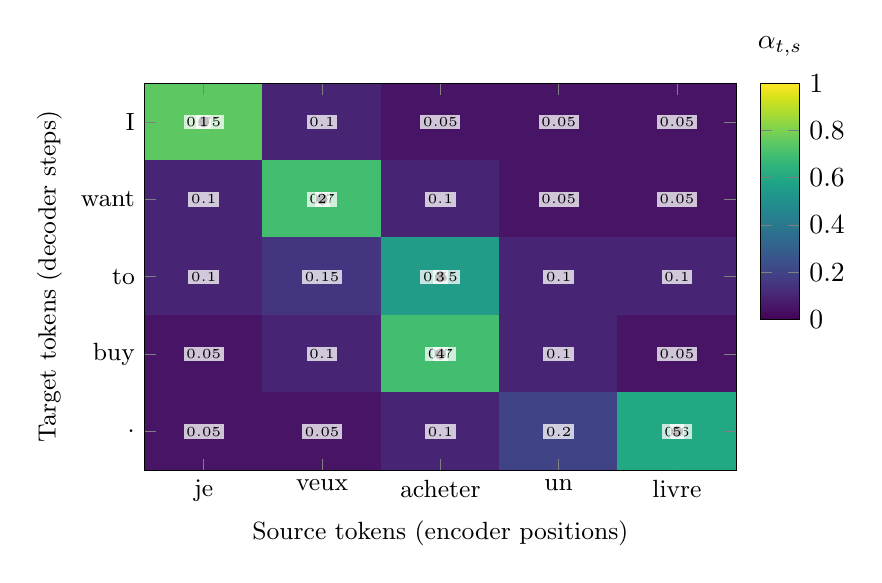
\begin{tikzpicture}
    \begin{axis}[
        width=0.75\linewidth,
        height=6.5cm,
        xlabel={Source tokens (encoder positions)},
        ylabel={Target tokens (decoder steps)},
        xtick={1,2,3,4,5},
        xticklabels={je, veux, acheter, un, livre},
        ytick={1,2,3,4,5},
        yticklabels={I, want, to, buy,.},
        y dir=reverse,
        colormap/viridis,
        colorbar,
        colorbar style={title={$\alpha_{t, s}$}, height=3.0cm},
        nodes near coords={\pgfmathprintnumber[fixed, precision=2]{\pgfplotspointmeta}},
        nodes near coords align={center},
        every node near coord/.append style={
            font=\tiny,
            fill=white,
            fill opacity=0.75,
            text opacity=1,
            inner sep=1pt
        },
        point meta min=0, point meta max=1,
        every axis/.append style={font=\small},
        enlargelimits=false,
        axis on top,
    ]
    % rows = target tokens, columns = source tokens
    \addplot[
        matrix plot*,
        mesh/cols=5,
        mesh/rows=5,
        point meta=explicit,
    ] table[row sep=\\, meta=z]{
    x y z\\
    % I
    1 1 0.75\\ 2 1 0.10\\ 3 1 0.05\\ 4 1 0.05\\ 5 1 0.05\\
    % want
    1 2 0.10\\ 2 2 0.70\\ 3 2 0.10\\ 4 2 0.05\\ 5 2 0.05\\
    % to
    1 3 0.10\\ 2 3 0.15\\ 3 3 0.55\\ 4 3 0.10\\ 5 3 0.10\\
    % buy
    1 4 0.05\\ 2 4 0.10\\ 3 4 0.70\\ 4 4 0.10\\ 5 4 0.05\\
    % .
    1 5 0.05\\ 2 5 0.05\\ 3 5 0.10\\ 4 5 0.20\\ 5 5 0.60\\
    };
    % highlight argmax per target token
    \addplot[only marks, mark=*, mark size=1.8pt] coordinates {
        (1,1)  % I -> je
        (2,2)  % want -> veux
        (3,3)  % to -> acheter
        (3,4)  % buy -> acheter
        (5,5)  %. -> livre
    };
    \end{axis}
    \end{tikzpicture}
    % Avoid inline math in captions; it wraps poorly in some EPUB renderers.
    \caption{Attention heatmap for a translation model. Rows are target tokens (decoder steps) and columns are source tokens (encoder positions). Each cell is an attention weight; the dot in each row marks the source position receiving the most attention. Use it when checking whether attention aligns to the intended source context.}
    \label{fig:lec7-attention}
\end{figure}


\subsection{Wrapping Up the Derivations}
\label{sec:rnn_wrapping_up_the_derivations}

This chapter develops the core ideas behind recurrent neural networks (RNNs) for sequence modeling. A canonical task is language modeling: predicting the next token from preceding context.

Recall that the goal is to estimate the conditional probability of a word \( w_t \) given the sequence of previous words \( w_1, w_2, \ldots, w_{t-1} \):
\begin{equation}
    P(w_t \mid w_1, w_2, \ldots, w_{t-1}).
\label{eq:auto_rnn_991224fcd0}
\end{equation}

This probability can be modeled using an RNN, which maintains a hidden state \( \mathbf{h}_t \) that summarizes the history up to time \( t \). A common indexing choice is: consume the current token \(w_t\) (as an embedding \(\mathbf{x}_t\)) and predict the \emph{next} token \(w_{t+1}\). This is equivalent to modeling \(P(w_t\mid w_{1: t-1})\) after a one-step shift.
\begin{align}
    \mathbf{h}_t &= f(\mathbf{h}_{t-1}, \mathbf{x}_t; \theta), \\
    P(w_{t+1} \mid w_1, \ldots, w_t) &= g(\mathbf{h}_t; \theta), \label{eq:rnn_output_prob}
\end{align}
where \( \mathbf{x}_t \) is the input representation (e.g., word embedding) of the word \( w_t \), \( f \) is the recurrent update function parameterized by \(\theta\), and \( g \) maps the hidden state to a probability distribution over the vocabulary. Because the hidden state is computed recursively, \(\mathbf{h}_t\) already aggregates information about the entire prefix \((w_1,\ldots, w_t)\); predicting \(w_{t+1}\) from \(\mathbf{h}_t\) therefore reflects the Markovian summary that RNNs maintain. Explicitly, repeatedly substituting \eqref{eq:rnn_hidden_state} reveals that \(\mathbf{h}_t=f(f(\cdots f(\mathbf{h}_0,\mathbf{x}_1),\ldots),\mathbf{x}_t)\), so no information is lost other than the compression inherent to the finite-dimensional state vector.

\paragraph{Training Objective}

The network is trained to maximize the likelihood of the observed sequences in a large corpus of text. Given a training sequence \( (w_1, w_2, \ldots, w_T) \), the log-likelihood is:
\begin{equation}
    \mathcal{L}(\theta) = \sum_{t=1}^{T-1} \log P(w_{t+1} \mid w_1, \ldots, w_t; \theta).
\label{eq:auto_rnn_1c468f5940}
\end{equation}

This objective encourages the model to assign high probability to the actual next word in the sequence, effectively learning the statistical structure of the language without explicit labeling of word relationships.

\paragraph{Self-supervised nature of language modeling}

A key insight is that no explicit labeling is required to train such models. The natural co-occurrence statistics of words in large corpora serve as implicit supervision. For example, the model learns that the word "juice" often follows "apple" because this pattern frequently appears in the training data. This is the essence of \emph{self-supervised} learning in NLP, where the prediction targets are created directly from the input sequence.

\paragraph{Input representations.}
The input \(\mathbf{x}_t\) is a numeric vector. In language modeling and other discrete-token problems, it is typically a token embedding produced by a learned lookup table. \Cref{chap:nlp} covers where those vectors come from (training objectives, evaluation, and audit considerations).

\subsubsection{Worked example: sentiment as a many-to-one decision}
\label{sec:rnn_sentiment_worked_example}

To make the sequence viewpoint concrete, consider a short review such as:
\emph{``This place is great.''}
In a sentiment classifier, we map the token sequence \((w_1,\ldots, w_T)\) to a single label \(y\in\{0,1\}\) (negative/positive). The recurrence consumes numeric inputs \(\mathbf{x}_t\) (one per token) and produces a final state \(\mathbf{h}_T\) that summarizes the sentence:
\begin{equation}
\mathbf{h}_t=f(\mathbf{h}_{t-1},\mathbf{x}_t;\theta),\qquad
\hat{y}=\sigma(\mathbf{w}^\top \mathbf{h}_T+b),
\label{eq:rnn_sentiment_many_to_one}
\end{equation}
where \(\sigma(\cdot)\) is the logistic sigmoid and \(\hat{y}\) is the predicted probability of the positive class.

This setup highlights a subtle but important dependency between \emph{representation} and \emph{generalization}. If tokens are treated as unrelated IDs (e.g., purely one-hot indicators), then ``great'' and ``awesome'' are orthogonal inputs: the model has no built-in reason to transfer evidence across similar words unless the training objective supplies a geometry that makes them nearby. In \Cref{chap:nlp}, we return to this same kind of task and show how learning word vectors from context gives the model a meaningful input space before any sequence model is applied.

\paragraph{Summary of the Modeling Pipeline}

\begin{enumerate}
    \item Collect a large corpus of text data.
    \item Tokenize the text into sequences of words.
    \item Represent words as embeddings (initialized from a lookup table that is \emph{learned jointly} with the network parameters).
    \item Use an RNN to process sequences and produce hidden states.
    \item Predict the next word probability distribution from the hidden state.
    \item Train the model by maximizing the likelihood of the observed sequences.
\end{enumerate}

\begin{tcolorbox}[summarybox, title={LSTM and GRU equations (compact)}]
\textbf{LSTM} (single layer):
\[
\begin{aligned}
    \mathbf{i}_t &= \sigma(\mathbf{x}_t\mathbf{W}_i+\mathbf{h}_{t-1}\mathbf{U}_i+\mathbf{b}_i), &
    \mathbf{f}_t &= \sigma(\mathbf{x}_t\mathbf{W}_f+\mathbf{h}_{t-1}\mathbf{U}_f+\mathbf{b}_f), \\
    \tilde{\mathbf{c}}_t &= \tanh(\mathbf{x}_t\mathbf{W}_c+\mathbf{h}_{t-1}\mathbf{U}_c+\mathbf{b}_c), &
    \mathbf{o}_t &= \sigma(\mathbf{x}_t\mathbf{W}_o+\mathbf{h}_{t-1}\mathbf{U}_o+\mathbf{b}_o), \\
    \mathbf{c}_t &= \mathbf{f}_t\odot \mathbf{c}_{t-1} + \mathbf{i}_t\odot \tilde{\mathbf{c}}_t, &
    \mathbf{h}_t &= \mathbf{o}_t\odot \tanh(\mathbf{c}_t).
\end{aligned}
\]
\textbf{GRU}:
\[
\begin{aligned}
    \mathbf{z}_t &= \sigma(\mathbf{x}_t\mathbf{W}_z+\mathbf{h}_{t-1}\mathbf{U}_z+\mathbf{b}_z), &
    \mathbf{r}_t &= \sigma(\mathbf{x}_t\mathbf{W}_r+\mathbf{h}_{t-1}\mathbf{U}_r+\mathbf{b}_r), \\
    \tilde{\mathbf{h}}_t &= \tanh(\mathbf{x}_t\mathbf{W}_h+(\mathbf{r}_t\odot\mathbf{h}_{t-1})\mathbf{U}_h+\mathbf{b}_h), &
    \mathbf{h}_t &= (1-\mathbf{z}_t)\odot \mathbf{h}_{t-1} + \mathbf{z}_t\odot \tilde{\mathbf{h}}_t.
\end{aligned}
\]
All gates are elementwise; $\sigma$ denotes the logistic sigmoid and $\odot$ the Hadamard product.

\paragraph{Notation note.} In the sequence\hyp{}model chapters, $\sigma(\cdot)$ always denotes the logistic sigmoid gate nonlinearity; when $\sigma$ is used without an argument (e.g., in earlier chapters for noise scales $\sigma^2$) it refers to a standard deviation. Context distinguishes these roles; see \Cref{app:notation_collisions} for the cross-chapter symbol index.
\end{tcolorbox}

\paragraph{Optional refresher (padding and autoencoders).}
For a 1D/2D convolution with input size \(n\), kernel size \(k\), stride \(s\), and padding \(p\), the output size is
\[
\left\lfloor \frac{n + 2p - k}{s} \right\rfloor + 1.
\]
When \(s=1\) and you want to preserve size, choose \(p=(k-1)/2\) for odd \(k\). For encoder intuition, recall that autoencoders map \(\mathbf{x}\mapsto\mathbf{z}\mapsto\hat{\mathbf{x}}\) with a reconstruction loss; the same compression intuition reappears in sequence encoders and attention models.

\begin{tcolorbox}[summarybox, title={Key takeaways}]
\begin{itemize}
    \item Language modeling is trained with self-supervision by maximizing next-token likelihood.
    \item Token vectors provide the numeric inputs; RNN hidden states encode context over time.
    \item Stability tools (clipping, gating, attention) enable long-range dependency modeling.
\end{itemize}

\medskip
\noindent\textbf{Minimum viable mastery.}
\begin{itemize}
    \item Define the next-token objective and relate cross-entropy, perplexity, and log-likelihood.
    \item Explain BPTT, truncation, and masking for variable-length sequences.
    \item Describe why gates help (information and gradient flow) and when attention is a practical alternative.
\end{itemize}

\noindent\textbf{Common pitfalls.}
\begin{itemize}
    \item Train/inference mismatch (teacher forcing without a decoding strategy that reflects it).
    \item Unstable gradients on long sequences (no clipping, poor initialization, or overly large learning rates).
    \item Incorrect padding masks that leak future tokens or contaminate the loss.
\end{itemize}
\end{tcolorbox}

\begin{tcolorbox}[summarybox, title={Exercises and lab ideas}]
\begin{itemize}
    \item Train a many-to-one sentiment classifier; plot gradient norms with and without clipping.
    \item Train a small LSTM language model; compare perplexity with/without weight tying and scheduled sampling.
    \item Empirically sweep \(\|\mathbf{W}_{hh}\|\) (spectral scaling) and reproduce vanishing/exploding behavior.
    \item Implement the masked, truncated-BPTT loop above and verify that pads do not affect the loss.
\end{itemize}

\medskip
\noindent\textbf{If you are skipping ahead.} Keep the loss/perplexity diagnostics and masking discipline from this chapter. \Cref{chap:transformers} changes the architecture, but the same evaluation traps and data-leakage risks remain.
\end{tcolorbox}

\medskip
\paragraph{Where we head next.} \Cref{chap:nlp} translates this sequence viewpoint into representation tooling: embedding objectives, neighborhood/analogy diagnostics, and deployment audits. Keep the sentiment example (\Cref{sec:rnn_sentiment_worked_example}) in mind: with learned token geometry, the same many\hyp{}to\hyp{}one task generalizes better than with raw IDs. \Cref{chap:transformers} then changes architecture again, replacing recurrence with attention while preserving the same evaluation and masking discipline.

\nocite{JurafskyMartin2023, Goodfellow2016, Mikolov2010, LevyGoldberg2014}
